\chapter{Scikit-NeuroMSI: Un Framework para Modelado de Integración Multisensorial}
\label{chapter:scikit_neuromsi}

El desarrollo de modelos computacionales de integración multisensorial ha sido tradicionalmente fragmentado, con diferentes grupos de investigación implementando sus propios modelos en diversos lenguajes y frameworks, dificultando la comparación sistemática y la reproducibilidad. Este capítulo presenta Scikit-NeuroMSI, el framework de código abierto en Python\footnote{\url{https://www.python.org/}} desarrollado por \citeauthor{paredes2025scikit}, que proporciona la infraestructura técnica sobre la cual se desarrolla el presente trabajo.

% =============================================================================
% SECCIÓN 1: MOTIVACIÓN Y OBJETIVOS
% =============================================================================

\section{Motivación y objetivos del framework}
\label{sec:snmsi_motivacion}

La integración multisensorial es un proceso neuronal fundamental que ha sido estudiado desde múltiples niveles de análisis, generando una diversidad de modelos teóricos. Sin embargo, hasta el desarrollo de Scikit-NeuroMSI, no existía un marco consolidado que facilitara la implementación, comparación y validación de estos modelos en contextos experimentales diversos \citep{paredes2025scikit}.

Los objetivos principales del framework son:

\begin{itemize}
\item Proporcionar una \textbf{infraestructura común} para implementar modelos de integración multisensorial a diferentes niveles de descripción, desde modelos probabilísticos de alto nivel hasta redes neuronales biológicamente inspiradas.

\item Facilitar la \textbf{comparación sistemática} entre modelos mediante interfaces estandarizadas para simulación y evaluación.

\item Promover la \textbf{reproducibilidad} de resultados computacionales en la comunidad de investigación en neurociencia computacional.

\item Servir como \textbf{plataforma educativa} para la enseñanza de conceptos de integración multisensorial y modelado neurocomputacional.
\end{itemize}

% =============================================================================
% SECCIÓN 2: ARQUITECTURA DE SOFTWARE
% =============================================================================

\section{Arquitectura de software}
\label{sec:snmsi_arquitectura}

Scikit-NeuroMSI está diseñado siguiendo principios de ingeniería de software que facilitan la extensibilidad y comparación entre modelos. La arquitectura se fundamenta en patrones de diseño establecidos que permiten agregar nuevos modelos sin modificar el código existente.

\subsection{Principios de diseño}
\label{subsec:snmsi_principios}

% ACAAAA: Se expandió la explicación del DIP para incluir los mecanismos concretos de implementación (metaclases, ParameterAliasTemplate, SKNMSIRunConfig)
El framework implementa el \textbf{Principio de Inversión de Dependencias} \acrfull{DIP}, donde los módulos de alto nivel no dependen de módulos de bajo nivel, sino que ambos dependen de abstracciones. Esto se logra mediante la definición de interfaces abstractas que especifican qué operaciones debe soportar cualquier modelo, independientemente de su implementación interna. 

Concretamente, el framework utiliza el mecanismo de metaclases de Python a través del método \texttt{\_\_init\_subclass\_\_}, que valida automáticamente que cada nueva subclase implemente todos los atributos y métodos requeridos. Esta validación en tiempo de definición de clase previene errores comunes y garantiza la conformidad con la interfaz esperada.

Adicionalmente, el framework utiliza el \textbf{Patrón Estrategia} (\textit{Strategy Pattern}), que permite encapsular diferentes algoritmos de integración sensorial como objetos intercambiables. Un usuario puede, por ejemplo, comparar las predicciones de un modelo bayesiano con las de una red neuronal simplemente intercambiando el objeto modelo, sin modificar el código de simulación o análisis.

% ACAAAA: Nueva subsección agregada para documentar el sistema de aliasing de parámetros, una característica distintiva del framework
\subsection{Sistema de aliasing de parámetros}
\label{subsec:snmsi_aliasing}

Una característica distintiva del framework es el sistema de \textbf{aliasing de parámetros}, implementado mediante la clase \texttt{ParameterAliasTemplate}. Este sistema permite que los modelos definan nombres genéricos internos para sus parámetros (como \texttt{mode0\_position}, \texttt{mode1\_position}), mientras que los usuarios pueden interactuar con nombres más intuitivos y específicos del dominio (como \texttt{auditory\_position}, \texttt{visual\_position}).

El aliasing se configura en tiempo de instanciación del modelo. Por ejemplo, al crear un modelo con \texttt{mode0="auditory"} y \texttt{mode1="visual"}, el sistema automáticamente genera los alias correspondientes, permitiendo que el método \texttt{run()} acepte parámetros como \texttt{auditory\_position} en lugar del genérico \texttt{mode0\_position}. Esta abstracción facilita la legibilidad del código de usuario sin sacrificar la generalidad interna del framework.

\subsection{Clases principales}
\label{subsec:snmsi_clases}

La arquitectura central se compone de varias clases principales que definen la estructura del framework:

% ACAAAA: Se corrigió "ModelABC" por "SKNMSIMethodABC" que es el nombre real de la clase en el código
\textbf{SKNMSIMethodABC} (\textit{Scikit-NeuroMSI Method Abstract Base Class}) es la clase base abstracta que define la interfaz estándar para todos los métodos de integración sensorial. Cualquier modelo que herede de esta clase puede ser procesado uniformemente por las herramientas del framework, independientemente de si es un modelo bayesiano, una red neuronal, o un estimador de máxima verosimilitud. Los atributos de clase que todo modelo debe definir incluyen: \texttt{\_run\_input} y \texttt{\_run\_output} (configuración de aliasing), \texttt{\_model\_type} (uno de ``MLE'', ``Bayesian'', o ``Neural''), y \texttt{\_output\_mode} (formato de salida). A nivel de instancia, debe implementar propiedades como \texttt{time\_range}, \texttt{position\_range}, \texttt{time\_res}, \texttt{position\_res}, y los métodos \texttt{run()} y \texttt{set\_random()}.

% ACAAAA: Se corrigió la descripción de dimensiones: no existe "trial" como dimensión, se especifican las 4 dimensiones reales del framework
\textbf{NDResult} (\textit{N-Dimensional Result}) es el objeto responsable de almacenar la información multidimensional de los estímulos y las respuestas del modelo. Esta estructura maneja datos con exactamente cuatro dimensiones predefinidas: \texttt{modes} (modalidades sensoriales como visual, auditiva, multisensorial), \texttt{times} (evolución temporal de las respuestas), \texttt{positions} (posiciones espaciales de los estímulos), y \texttt{positions\_coordinates} (coordenadas múltiples para cada posición, útil en espacios multidimensionales). NDResult proporciona además herramientas integradas para el análisis de resultados mediante \textit{accessors} al estilo de pandas: \texttt{result.plot} para visualización y \texttt{result.stats} para estadísticas descriptivas. La exportación a formatos estándar se realiza mediante el método \texttt{to\_ndr()}.


% ACAAAA: Se expandió la descripción de NDResultCollection para incluir los accessors específicos que provee
\textbf{NDResultCollection} permite agregar múltiples objetos NDResult, facilitando el análisis de barridos de parámetros o comparaciones entre modelos. Esta clase implementa operaciones de filtrado, agrupamiento y reducción sobre colecciones de resultados. Proporciona accessors especializados: \texttt{bias\_acc} para cálculo de sesgos cross-modales, \texttt{causes\_acc} para análisis de inferencia causal, y \texttt{cplot\_acc} para visualización a nivel de colección. Similar a NDResult, ofrece la capacidad de exportar los datos mediante el método \texttt{to\_ndc()}.

% ACAAAA: Se expandió la descripción de ParameterSweep para incluir manejo de memoria, paralelización y el argumento repeat
\textbf{ParameterSweep} es una herramienta para realizar barridos sistemáticos de parámetros sobre cualquier modelo. Dado un modelo y un conjunto de rangos para sus parámetros, ParameterSweep ejecuta automáticamente simulaciones para todas las combinaciones especificadas, almacenando los resultados en una NDResultCollection para análisis posterior. La clase implementa estrategias de procesamiento intercambiables mediante \texttt{ProcessingStrategyABC}, soporta ejecución paralela mediante \texttt{joblib}, y proporciona control de memoria con advertencias (\texttt{MaybeTooBigForAvailableMemoryWarning}) y errores (\texttt{ToBigForAvailableMemoryError}) cuando los resultados exceden la memoria disponible. El parámetro \texttt{repeat} permite ejecutar múltiples repeticiones (trials) de cada condición experimental.

% ACAAAA: Se corrigió el label de la figura que decía "fig:feed-forward" (no relacionado) por "fig:arquitectura-sknmsi"
\begin{figure}[H]
    \centering
    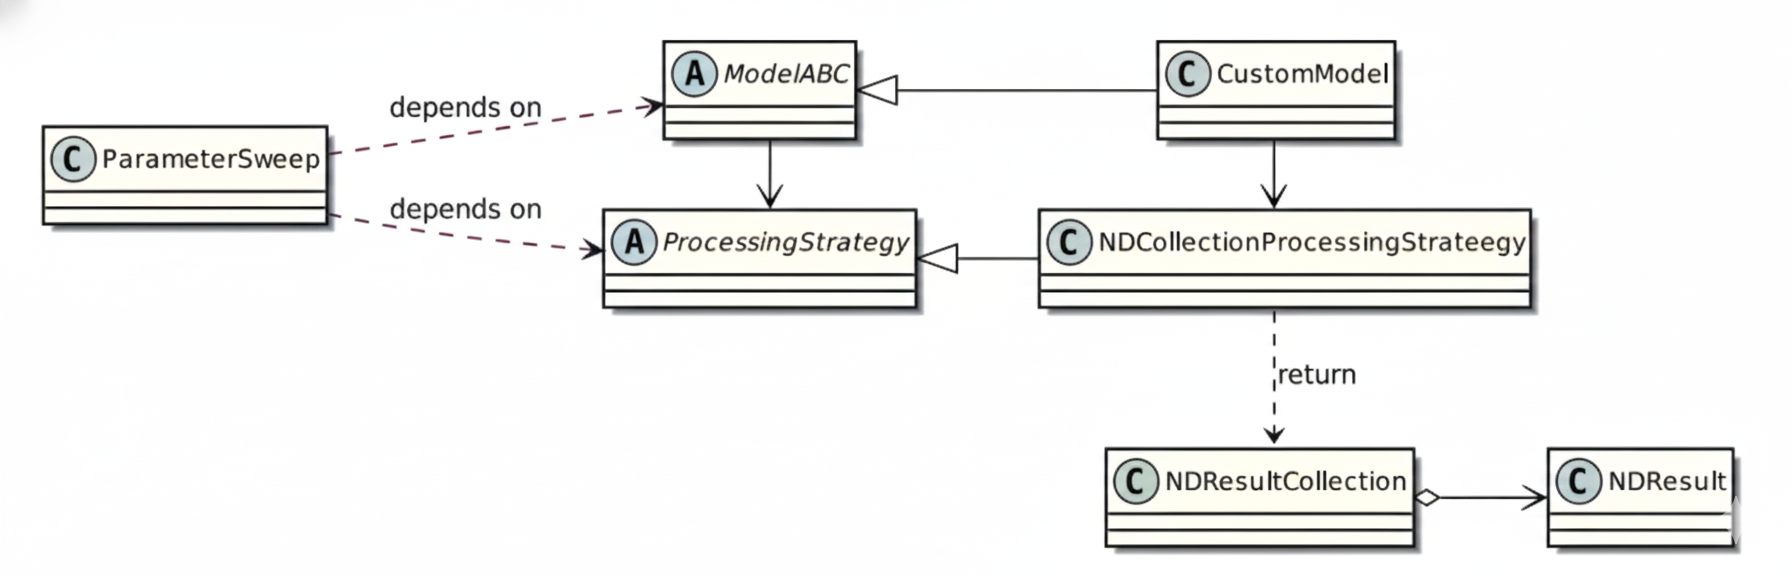
\includegraphics[width=0.55\textwidth]{06_neuromsi/figures/arqui-neuromsi.png}
    \caption{
        Diagrama de clases reducido de Scikit-NeuroMSI. Las flechas vacías representan la herencia, la flecha con punta de diamante indica que varios objetos NDResult se agregan en una única NDResultCollection, y todas las demás relaciones tienen etiquetas explicativas.
    }
    \label{fig:arquitectura-sknmsi}
\end{figure}

\subsection{Backend de datos}
\label{subsec:snmsi_backend}

El almacenamiento y manipulación de datos multidimensionales se implementa mediante \textbf{XArray}\footnote{\url{https://docs.xarray.dev/en/stable/}}, una biblioteca de Python diseñada específicamente para trabajar con arreglos etiquetados de N dimensiones. Esta extiende las capacidades de NumPy agregando nombres y coordenadas a cada dimensión, lo que facilita la selección, agregación y visualización de datos complejos.

% ACAAAA: Se corrigió la descripción del formato de archivos: son archivos ZIP que contienen JSON (metadatos) + NetCDF (datos), no solo "NetCDF con convenciones"
Para la persistencia de datos, el framework utiliza un formato basado en archivos ZIP que combina \acrfull{NetCDF} para los datos multidimensionales con JSON para los metadatos. Los resultados de simulaciones se guardan en archivos con extensión \textbf{.ndr} (\textit{NDResult}) o \textbf{.ndc} (\textit{NDResultCollection}). Internamente, cada archivo ZIP contiene: \texttt{metadata.json} con información del modelo, parámetros de ejecución, versión del framework, plataforma y timestamp; y \texttt{nddata.nc} con los datos xarray en formato NetCDF. Esta estructura permite que los resultados sean cargados y analizados posteriormente, compartidos entre investigadores, o procesados con herramientas externas compatibles con NetCDF.

% ACAAAA: Nueva subsección agregada para documentar el sistema de compresión de resultados
\subsection{Sistema de compresión}
\label{subsec:snmsi_compresion}

Para manejar eficientemente grandes volúmenes de datos, el framework proporciona un sistema de compresión mediante las funciones \texttt{compress\_ndresult()} y \texttt{decompress\_ndresult()}, que producen objetos \texttt{CompressedNDResult}. Este sistema permite almacenar resultados en memoria de forma compacta cuando no se requiere acceso frecuente a los datos, y descomprimirlos bajo demanda para análisis. Los parámetros de compresión son configurables mediante \texttt{DEFAULT\_COMPRESSION\_PARAMS} y validables con \texttt{validate\_compression\_params()}.

% =============================================================================
% SECCIÓN 3: MODELOS IMPLEMENTADOS
% =============================================================================

\section{Modelos implementados}
\label{sec:snmsi_modelos}

El framework incluye implementaciones de referencia de varios modelos establecidos en la literatura de integración multisensorial. Estas implementaciones sirven tanto como herramientas de investigación como ejemplos para desarrolladores que deseen agregar nuevos modelos.

% ACAAAA: Se agregó una tabla resumen de todos los modelos implementados con sus características
\begin{table}[H]
\centering
\caption{Modelos implementados en Scikit-NeuroMSI. La columna ``Tipo'' indica la categoría del modelo según la clasificación del framework.}
\label{tab:modelos_sknmsi}
\begin{tabular}{llll}
\hline
\textbf{Clase} & \textbf{Tipo} & \textbf{Referencia} & \textbf{Dinámica temporal} \\
\hline
\texttt{AlaisBurr2004} & MLE & \citet{alais2004ventriloquist} & No \\
\texttt{Kording2007} & Bayesian & \citet{kording2007causal} & No \\
\texttt{Zhu2024} & Bayesian & \citet{zhu2024bci} & No \\
\texttt{Cuppini2014} & Neural & \citet{cuppini2014neural} & Sí (ODE) \\
\texttt{Cuppini2017} & Neural & \citet{cuppini2017biologically} & Sí (ODE) \\
\texttt{Paredes2025} & Neural & \citet{paredes2025scikit} & Sí (ODE) \\
\texttt{Echeveste2020} & Neural & \citet{echeveste2020cortical} & Sí (SDE) \\
\hline
\end{tabular}
\end{table}

\subsection{Modelos de máxima verosimilitud}
\label{subsec:snmsi_mle}

% ACAAAA: Se cambió "integrador bimodal óptimo" por el nombre real de la clase "AlaisBurr2004" y se estructuró como subsección
El modelo \textbf{AlaisBurr2004} implementa la combinación de señales mediante máxima verosimilitud según las ecuaciones presentadas en la Sección~\ref{subsec:integracion_optima}. Este modelo asume que ambas señales sensoriales provienen de la misma fuente y las combina ponderando por sus confiabilidades relativas (inversas de las varianzas).

La implementación permite especificar las varianzas de las señales visual y auditiva, ya sea como valores fijos o como funciones de la posición espacial (capturando, por ejemplo, la menor precisión auditiva en la periferia). El modelo proporciona una línea base teórica contra la cual comparar modelos más complejos.

\subsection{Modelos bayesianos}
\label{subsec:snmsi_bayesianos}

% ACAAAA: Se reestructuró como subsección y se agregó mención del modelo Zhu2024 que faltaba
El modelo \textbf{Kording2007} implementa el marco de inferencia causal bayesiana de \citet{kording2007causal} para inferir la estructura causal subyacente a las señales multisensoriales. A diferencia del integrador MLE, este modelo no asume automáticamente que las señales provienen de la misma fuente, sino que computa la probabilidad posterior de causa común versus causas separadas.

La implementación incluye el cálculo de la probabilidad de causa común, el promediado bayesiano sobre estructuras causales \acrfull{BMA}, y la generación de respuestas de sesgo de localización y juicio de unidad. Los parámetros ajustables incluyen la probabilidad prior de causa común y las varianzas sensoriales.

% ACAAAA: Se agregó el modelo Zhu2024 que no estaba documentado
El modelo \textbf{Zhu2024} proporciona una implementación alternativa de inferencia causal bayesiana basada en el BCI Toolbox \citep{zhu2024bci}. Esta implementación ofrece funcionalidades adicionales y puede servir como referencia para validar resultados con la implementación de Körding.

\subsection{Modelos de redes neuronales}
\label{subsec:snmsi_neurales}

% ACAAAA: Se agregó el modelo Cuppini2014 que no estaba documentado
El modelo \textbf{Cuppini2014} implementa una arquitectura de red neuronal de dos capas (auditiva y visual) con conectividad lateral tipo sombrero mexicano y conexiones cross-modales. Esta implementación representa el modelo base del cual deriva la versión extendida de 2017.

% ACAAAA: Se reestructuró la descripción de Cuppini2017 como párrafo dentro de la subsección
El modelo \textbf{Cuppini2017} proporciona una implementación completa de la arquitectura de tres capas descrita en la Sección~\ref{sec:modelo_cuppini}. Esta implementación permite simular la dinámica temporal del modelo mediante integración de ecuaciones diferenciales ordinarias (ODE) usando BrainPy como backend. Los parámetros configurables incluyen los pesos de conexiones cross-modales, la amplitud de las conexiones laterales tipo sombrero mexicano, y las constantes de tiempo de las diferentes capas. La implementación soporta la presentación de estímulos audiovisuales con disparidades espaciales y temporales configurables, y extrae predicciones sobre el efecto ventrílocuo (sesgo de localización auditiva) y la inferencia causal (número de picos en la capa multisensorial).

% ACAAAA: Se reestructuró la descripción de Paredes2025 (antes "red espacio-temporal") con su nombre de clase correcto
El modelo \textbf{Paredes2025} extiende la red de Cuppini para incorporar disparidades temporales además de espaciales. Permite estudiar la ventana de integración temporal, es decir, el rango de asincronías audiovisuales dentro del cual los estímulos se perciben como provenientes de una fuente común.

La implementación incluye filtros temporales diferenciados para las modalidades visual y auditiva, capturando las diferentes latencias de procesamiento. Esto permite simular fenómenos como la ilusión del flash inducido por sonido (\textit{sound-induced flash illusion}), donde un único flash acompañado de múltiples sonidos se percibe como múltiples flashes.

% ACAAAA: Se agregó la descripción del modelo Echeveste2020 que es la contribución principal de esta tesis
El modelo \textbf{Echeveste2020} implementa una red neuronal estabilizada supralinear (SSN) que realiza inferencia probabilística mediante muestreo estocástico, como se describe en detalle en el Capítulo~\ref{chapter:echeveste}. A diferencia de los modelos anteriores que usan ecuaciones diferenciales ordinarias, este modelo utiliza ecuaciones diferenciales estocásticas (SDE), lo que le permite representar la variabilidad neuronal de manera natural. La implementación incluye 50 canales de orientación (-90° a 90°), poblaciones excitatorias e inhibitorias, y conectividad estructurada según estadísticas de imágenes naturales. Este modelo representa la contribución principal del presente trabajo al framework.

% =============================================================================
% ACAAAA: Nueva sección agregada para documentar el módulo generativo (GSM) que es fundamental para Echeveste2020
% =============================================================================


% TODO ESTO PARA LA PROXIMA SECCION

\section{Modelos generativos}
\label{sec:snmsi_generativos}

Además de los modelos de integración, el framework incluye un módulo de modelos generativos (\texttt{skneuromsi.generative}) diseñado para generar estímulos con propiedades estadísticas realistas.

\subsection{Gaussian Scale Mixture (GSM)}
\label{subsec:snmsi_gsm}

La clase \textbf{GSM} implementa el modelo generativo de Mezcla Gaussiana de Escalas utilizado para modelar las estadísticas de imágenes naturales \citep{wainwright1999scale}. Este modelo es fundamental para el funcionamiento de Echeveste2020, ya que define la distribución a priori sobre los estímulos visuales.

La implementación permite:
\begin{itemize}
    \item Generar bancos de filtros de Gabor con orientaciones y frecuencias espaciales configurables.
    \item Calcular matrices de covarianza a partir de parches de imágenes naturales.
    \item Generar estímulos sintéticos que siguen las estadísticas aprendidas.
    \item Blanquear estímulos para preprocesamiento.
\end{itemize}

La función de fábrica \texttt{create\_echeveste\_gsm()} proporciona una instancia preconfigurada con los parámetros utilizados en \citet{echeveste2020cortical}: 50 orientaciones, parches de 16×16 píxeles, frecuencia espacial de 0.2 ciclos/píxel, y ancho de banda de 1 octava.

% =============================================================================
% ACAAAA: Nueva sección agregada para documentar los parámetros pre-entrenados incluidos en el framework
% =============================================================================

% esto tambien para la nueva seccion

\section{Datos y parámetros pre-entrenados}
\label{sec:snmsi_datos}

El framework incluye un módulo de datos (\texttt{skneuromsi.data}) que proporciona acceso a parámetros pre-entrenados para los modelos más complejos.

\subsection{Parámetros de Echeveste2020}
\label{subsec:snmsi_datos_echeveste}

La clase \textbf{EchevesteDataLoader} proporciona acceso a los parámetros optimizados del modelo Echeveste2020:

\begin{itemize}
    \item \textbf{Parámetros del GSM}: Matriz de filtros de Gabor ($\mathbf{A}$, 256×50) y matriz de covarianza a priori ($\mathbf{C}$, 50×50).

    \item \textbf{Parámetros de conectividad SSN}: Ocho parámetros que definen la estructura de conexiones entre poblaciones ($a_{EE}$, $a_{EI}$, $a_{IE}$, $a_{II}$ para amplitudes y $d_{EE}$, $d_{EI}$, $d_{IE}$, $d_{II}$ para anchos espaciales).

    \item \textbf{Parámetros de transformación de entrada}: Tres parámetros ($\alpha_h$, $\beta_h$, $\gamma_h$) que controlan cómo el input del GSM se transforma en corriente de entrada a la red.

    \item \textbf{Parámetros de covarianza de ruido}: Cuatro parámetros ($\sigma_E^2$, $\sigma_I^2$, $\sigma_{width}$, $\rho$) que definen la estructura espacial del ruido inyectado.
\end{itemize}

Estos parámetros fueron optimizados para que los momentos de la actividad de la red reproduzcan los momentos objetivo derivados de la inferencia probabilística exacta, como se describe en la Sección~\ref{sec:echeveste_entrenamiento}.

% =============================================================================
% SECCIÓN 5: IMPLEMENTACIÓN TÉCNICA
% =============================================================================

\section{Implementación técnica}
\label{sec:snmsi_implementacion}

Esta sección describe aspectos técnicos de la implementación relevantes para desarrolladores que deseen extender el framework o comprender su funcionamiento interno.

\subsection{Gestión de dependencias}
\label{subsec:snmsi_dependencias}

% ACAAAA: Se corrigió la lista de dependencias para incluir BrainPy (crítico para modelos neuronales) y joblib (para paralelización)
Scikit-NeuroMSI está implementado en Python 3 y depende de bibliotecas estándar del ecosistema científico: NumPy para operaciones numéricas, SciPy para algoritmos científicos, XArray para datos multidimensionales, Matplotlib y Seaborn para visualización, pandas para manipulación de datos tabulares, joblib para paralelización, y tqdm para barras de progreso. Para los modelos neuronales con dinámica temporal, el framework utiliza \textbf{BrainPy}\footnote{\url{https://brainpy.readthedocs.io/}} como backend de integración numérica, que opcionalmente soporta aceleración mediante JAX para cómputo en GPU.

El framework se distribuye a través de PyPI (\textit{Python Package Index}), permitiendo instalación mediante \texttt{pip install scikit-neuromsi}. Las dependencias se gestionan automáticamente durante la instalación.

% ACAAAA: Nueva subsección agregada para documentar la configuración de dispositivos (GPU/CPU)
% esto tmb es nuevo

\subsection{Configuración de dispositivos}
\label{subsec:snmsi_dispositivos}

Para modelos que soportan aceleración por GPU, el framework proporciona utilidades de configuración de dispositivos mediante el módulo \texttt{skneuromsi.neural}:

\begin{itemize}
    \item \texttt{DeviceConfig}: Clase que encapsula la configuración del dispositivo de cómputo.
    \item \texttt{configure\_device()}: Función para establecer el dispositivo (CPU o GPU específica).
    \item \texttt{get\_device\_config()}: Función para consultar la configuración actual.
\end{itemize}

Esta abstracción permite que el código de usuario sea agnóstico al hardware subyacente, facilitando la portabilidad entre diferentes entornos de ejecución.

\subsection{Ejecución paralela}
\label{subsec:snmsi_paralelo}

% ACAAAA: Se corrigió: el framework usa joblib, no multiprocessing directamente
Para barridos de parámetros extensos, el framework soporta ejecución paralela mediante la biblioteca \texttt{joblib}. El usuario puede especificar el número de procesos a utilizar, y el framework distribuye automáticamente las simulaciones entre ellos.

Para modelos implementados con JAX a través de BrainPy, la paralelización puede extenderse a GPUs mediante las primitivas de JAX, permitiendo ejecutar múltiples simulaciones simultáneamente en dispositivos de alto rendimiento.

\subsection{Gestión de memoria}
\label{subsec:snmsi_memoria}

Los modelos de redes neuronales con dinámica temporal pueden generar grandes volúmenes de datos (actividad de cientos de neuronas durante miles de pasos temporales en múltiples trials). El framework implementa estrategias para manejar estos casos: almacenamiento incremental a disco durante simulaciones largas, compresión de datos mediante el sistema \texttt{CompressedNDResult} descrito en la Sección~\ref{subsec:snmsi_compresion}, y opciones para almacenar solo estadísticas resumidas en lugar de trayectorias completas.

% =============================================================================
% SECCIÓN 6: APLICACIONES
% =============================================================================

\section{Aplicaciones}
\label{sec:snmsi_aplicaciones}

En el artículo que presenta el framework, \citet{paredes2025scikit} demuestran su utilidad mediante varios análisis representativos.

\subsection{Paradigma del efecto ventrílocuo}
\label{subsec:snmsi_ventrilocuo}

El efecto ventrílocuo, introducido en la Sección~\ref{subsec:ventriloquismo}, constituye el paradigma principal para validar modelos de integración audiovisual. El framework permite simular experimentos típicos donde estímulos visual y auditivo se presentan con diferentes disparidades espaciales, midiendo el sesgo resultante en la localización auditiva percibida.

% ACAAAA: Se agregó un ejemplo de código básico para ilustrar el uso típico del framework
Un ejemplo típico de uso del framework para simular el efecto ventrílocuo es:

\begin{verbatim}
from skneuromsi.neural import Cuppini2017
from skneuromsi import ParameterSweep
import numpy as np

# Crear modelo con modalidades específicas
model = Cuppini2017(mode0="auditory", mode1="visual")

# Configurar barrido de disparidades
disparities = np.arange(-24, 25, 6)
sweep = ParameterSweep(
    model=model,
    target="visual_position",
    range=45 + disparities
)

# Ejecutar simulaciones
results = sweep.run(auditory_position=45)

# Visualizar resultados
results.cplot.unity_report()
\end{verbatim}

Los autores comparan las predicciones de modelos bayesianos y de redes neuronales, encontrando que ambos reproducen cualitativamente el patrón experimental de sesgo decreciente con la disparidad, pero con diferencias cuantitativas que podrían distinguirse experimentalmente.

\subsection{Ilusión del flash inducido por sonido}
\label{subsec:snmsi_flash}

Esta ilusión, donde un único flash visual acompañado de múltiples sonidos se percibe como múltiples flashes, demuestra que la integración multisensorial puede alterar la percepción incluso de modalidades típicamente dominantes como la visión. El modelo Paredes2025, desarrollado por el grupo de investigación de los autores del framework, fue construido específicamente para dar cuenta de este fenómeno \citep{paredes2025scikit}.


\subsection{Aplicaciones clínicas}
\label{subsec:snmsi_clinicas}

Los autores señalan que una aplicación prometedora del framework es el estudio de diferencias en integración multisensorial asociadas a condiciones psiquiátricas y neurológicas. Estudios han documentado alteraciones en la integración audiovisual en trastornos del espectro autista (TEA), esquizofrenia, y demencias. El framework permitiría formalizar hipótesis sobre qué parámetros de los modelos podrían estar alterados en estas condiciones, y generar predicciones cuantitativas testables experimentalmente.

% =============================================================================
% SECCIÓN 7: COMPARACIÓN CON OTROS FRAMEWORKS
% =============================================================================

\section{Contexto en el ecosistema de herramientas}
\label{sec:snmsi_contexto}

Scikit-NeuroMSI ocupa un nicho específico en el ecosistema de herramientas para neurociencia computacional. A diferencia de simuladores de redes neuronales de propósito general como \textbf{Brian}\footnote{\url{https://briansimulator.org/}} o \textbf{NEST}\footnote{\url{https://ebrains.eu/data-tools-services/tools/nest}}, que se enfocan en la simulación detallada de neuronas de disparo, Scikit-NeuroMSI está diseñado específicamente para modelos de integración multisensorial, proporcionando abstracciones y herramientas optimizadas para este dominio.

Comparado con frameworks de modelado cognitivo como \textbf{HDDM}\footnote{\url{https://hddm.readthedocs.io/}} (para modelos de difusión de decisiones) o \textbf{TAPAS}\footnote{\url{https://www.translationalneuromodeling.org/tapas}} (para modelos computacionales en psiquiatría), Scikit-NeuroMSI se especializa en la dimensión sensorial del procesamiento, permitiendo una descripción más detallada de cómo señales de múltiples modalidades se combinan antes de informar decisiones.

% ACAAAA: Se corrigió la mención de BrainPy ya que ahora es una dependencia del framework, no un competidor
Frameworks de redes neuronales recurrentes como \textbf{PyRates}\footnote{\url{https://pyrates.readthedocs.io/}} comparten el enfoque en dinámicas de poblaciones neuronales, pero no incluyen las abstracciones específicas para estímulos multisensoriales, inferencia causal, o métricas de integración que Scikit-NeuroMSI proporciona. Cabe destacar que Scikit-NeuroMSI utiliza \textbf{BrainPy} como backend para la integración numérica de sus modelos neuronales, aprovechando sus capacidades de diferenciación automática y aceleración por GPU.

% =============================================================================
% SECCIÓN 8: DIRECCIONES FUTURAS Y CONTRIBUCIONES
% =============================================================================

\section{Direcciones futuras y contribuciones de la comunidad}
\label{sec:snmsi_futuro}

El desarrollo de Scikit-NeuroMSI continúa activamente, con varias direcciones planificadas para versiones futuras.

\subsection{Mejoras arquitectónicas}
\label{subsec:snmsi_mejoras}

Una mejora planificada es la separación más clara entre la representación de estímulos y los integradores que los procesan. Actualmente, algunos modelos asumen formatos específicos de estímulo, lo que limita la flexibilidad. Una arquitectura de ``estímulo-integrador'' más modular permitiría combinar diferentes tipos de estímulos con diferentes modelos de manera más flexible.

Otra dirección es el soporte mejorado para modelos jerárquicos, donde la salida de un modelo alimenta la entrada de otro. Esto permitiría construir arquitecturas complejas combinando componentes más simples.

\subsection{Nuevos modelos}
\label{subsec:snmsi_nuevos_modelos}

El framework está diseñado para que la comunidad contribuya nuevas implementaciones de modelos. Dando lugar al presente trabajo que contribuye en esta dirección mediante la implementación del modelo de Echeveste, que introduce al framework el primer modelo con dinámicas corticales realistas basadas en muestreo estocástico. Esta implementación establece patrones para que futuros contribuidores puedan seguir para agregando modelos similares.

\subsection{Información del proyecto}
\label{subsec:snmsi_info}

Scikit-NeuroMSI se distribuye bajo licencia BSD 3-Clause, permitiendo uso libre tanto académico como comercial. El código fuente está disponible en GitHub\footnote{\url{https://github.com/renatoparedes/scikit-neuromsi}}, donde se aceptan contribuciones mediante pull requests. La documentación completa, incluyendo tutoriales y referencia de API, está disponible en Read the Docs\footnote{\url{https://scikit-neuromsi.readthedocs.io}}.

% =============================================================================
% SECCIÓN 9: RELEVANCIA PARA EL PRESENTE TRABAJO
% =============================================================================

\section{Relevancia para el presente trabajo}
\label{sec:snmsi_relevancia}

Scikit-NeuroMSI proporciona la infraestructura técnica fundamental sobre la cual se desarrolla la implementación del modelo de Echeveste presentada en esta tesis. Específicamente:

La implementación existente del modelo de Cuppini sirve como \textbf{punto de referencia} para entender cómo modelos de redes neuronales se integran en el framework, y como objetivo eventual para futuras extensiones que combinen ambos enfoques.

La arquitectura modular del framework permite \textbf{integrar} el modelo de Echeveste de manera que pueda ser comparado directamente con modelos existentes usando las mismas herramientas de análisis.

% ACAAAA: Se corrigió: no existe dimensión "trial", se manejan mediante repeticiones en ParameterSweep
Las abstracciones de NDResult y XArray proporcionan una \textbf{estructura natural} para almacenar las trayectorias temporales de potenciales de membrana que el modelo de Echeveste genera, con soporte para múltiples condiciones de estímulo y poblaciones neuronales. Las repeticiones experimentales (trials) se manejan mediante el parámetro \texttt{repeat} de ParameterSweep, almacenándose como elementos individuales en NDResultCollection.

Las herramientas de visualización y análisis existentes pueden \textbf{extenderse} para las necesidades específicas del modelo de Echeveste, como análisis espectral para detectar oscilaciones gamma o comparación de momentos de respuesta con momentos objetivo.

Finalmente, al contribuir la implementación del modelo de Echeveste al framework, este trabajo la hace \textbf{disponible para la comunidad científica}, maximizando su impacto y reproducibilidad, y estableciendo las bases para que otros investigadores construyan sobre este trabajo hacia modelos de integración multisensorial con dinámicas corticales realistas.
